\section{Model Description}

The Bore Angle Calculation model uses vector mathematics in order to calculate the miss angle from a boresight on the spacecraft to its desired target. The model also calculates the azimuth angle of the boresight.

\begin{figure}[H]
	\centerline{
		 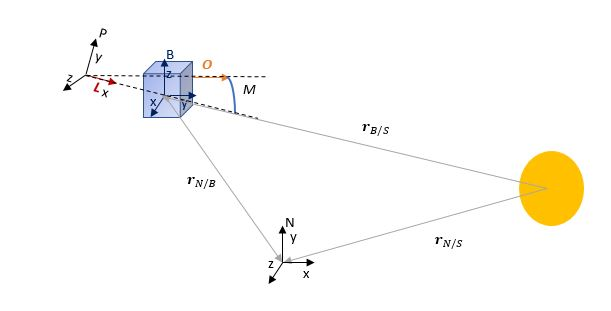
\includegraphics[height = 3in]{Figures/missAngleImg.JPG}
	}
	\caption{All of the vectors and the miss angle are labeled here. $\bm O$ is the vector that represents the boresight of the instrument that the test is interested in. $\bm{L}$ is the direction that the spacecraft should be pointing its boresight in. $\bm M$ is the miss angle of the boresight to its desired direction. All of the $\bm r$ vectors are various position vectors designated by their subscripts.} 
	\label{fig:Fig1}
\end{figure}

The model begins by creating a direction cosine martix to represent the pointing frame from the inertial frame. Then the boresight vector is projected into this frame, and the miss angle and the azimuth angle are calculated using standard trigonometry. These calculations are performed in the following way:

First, the unit relative position vector of the spacecraft is calculated relative to the celestial body that the spacecraft is supposed to be pointing at. Using Equation \ref{eq:rePos}. Where $\hat{\bm r}_{B/S}$ is the unit relative position of the spacecraft to the planet, $\bm r_{N/S}$ is the position of the celestial body in the inertial frame, and $\bm r_{N/B}$ is the position of the spacecraft in the inertial frame. 

 \begin{equation}
 	\label{eq:rePos}
 	\hat{\bm r}_{B/S} = \frac{\bm r_{N/S} - \bm r_{N/B}}{\vert \bm r_{N/S} - \bm r_{N/B} \vert}
\end{equation}

Next, the unit relative velocity of the spacecraft is calculated in the same manner.

 \begin{equation}
 	\label{eq:reVel}
 	\hat{\bm v}_{B/S} = \frac{\bm v_{N/S} - \bm v_{N/B}}{\vert \bm v_{N/S} - \bm v_{N/B} \vert}
\end{equation}

Then, direction cosine matrix from the pointing frame to the inertial frame is constructed. The first row of the direction cosine matrix is set to be the unit relative position vector calculated in the first step. The last row of the direction cosine matrix is set to be the result of the cross product of the relative unit position vector with the cross product of the relative position vector with the relative velocity vector. Then, the second row of the direction cosine matrix is set to be the cross product of the first and last row of the direction cosine matrix, as show in Equation \ref{eq:dcm3}

 \begin{equation}
 	\label{eq:dcm3}
 	[\bm{PN}] =  \begin{bmatrix}
    \hat{ \bm r}_{B/S}^T \\
    \hat{ \bm r}_{B/S} \times (\hat{\bm r}_{B/S}  \times  (\bm r_{B/S}  \times \bm v_{B/S})) ^T\\
    (\hat{\bm r}_{B/S}  \times  (\bm r_{B/S}  \times \bm v_{B/S}))^T
    \end{bmatrix}
\end{equation}

 Once the direction cosine matrix has been created, the direction cosine matrix from the body frame to the pointing frame is created by multiplying the direction cosine matrix from the body frame to the inertial frame and the inertial frame to the pointing frame together. Then the boresight vector, $\bm O$ (which is shown in Figure \ref{fig:Fig1}), is projected into the pointing frame by dotting the new direction cosine matrix with the boresight vector in the body frame. This is shown in Equation \ref{eq:boreSight}.

 \begin{equation}
 	\label{eq:boreSight}
 	\leftexp{P}{\bm {O}} = [\bm{PB}] \cdot\leftexp{B}{\bm {O}}
\end{equation}

From there, the boresight vector is multiplied by the baseline vector in the pointing frame. Where the baseline vector in the pointing frame is defined as $\bm L = \hat{\bm i}$. Then the product of the boresight vector and the baseline vector is passed through the arccosine function to get the boresight miss angle. As shown in Equation \ref{eq:missAng}.

 \begin{equation}
 	\label{eq:missAng}
 	M = \arccos(\bm O \cdot \bm L)
\end{equation}

\begin{figure}[H]
	\centerline{
		 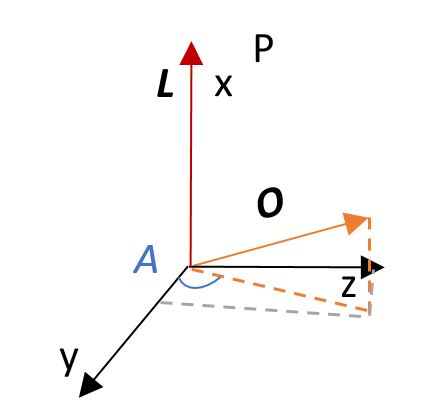
\includegraphics[height = 2.5in]{Figures/azi.JPG}
	}
	\caption{The azimuth angle, A is shown here with respect to the pointing coordinate frame and the vectors used to construct the azimuth angle.}
	\label{fig:Fig2}
\end{figure}
 
The azimuth angle is calculated by passing the product of the last two components of the borsight vector. This is shown in Equation \ref{eq:azAng} and in Figure \ref{fig:Fig2}.

 \begin{equation}
 	\label{eq:azAng}
 	A = \arctan(\bm O_{\hat k} \cdot \bm O_{\hat j})
\end{equation}